% Interaction diagram, LaTeX user level and TeX system software level
% Author: Agostino De Marco
% Based on diagram from Marco Miani and Pascal Seppecher.
\documentclass{article}
\usepackage{tikz}
%%%<
\usepackage{verbatim}
\usepackage[active,tightpage]{preview}
\PreviewEnvironment{tikzpicture}
\setlength\PreviewBorder{5pt}%
%%%>
\usetikzlibrary{positioning}

\newcommand{\yslant}{0.5}
\newcommand{\xslant}{-0.6}
\begin{document}
\begin{tikzpicture}[scale=1.1,every node/.style={minimum size=1cm},on grid]

	% system level
	\begin{scope}[
		yshift=-120,
		every node/.append style={yslant=\yslant,xslant=\xslant},
		yslant=\yslant,xslant=\xslant
	] 
		% The lower frame:
		\draw[black, dashed, thick] (-3,0) rectangle (3,4.8); 
		% Agents:
		\draw[fill=red]  
			(-0.5,2) circle (.1); % .tex file
		% Flows:
		\node[anchor=south,inner sep=0,xshift=2pt,yshift=-5pt,fill=white] at (0,2)
		{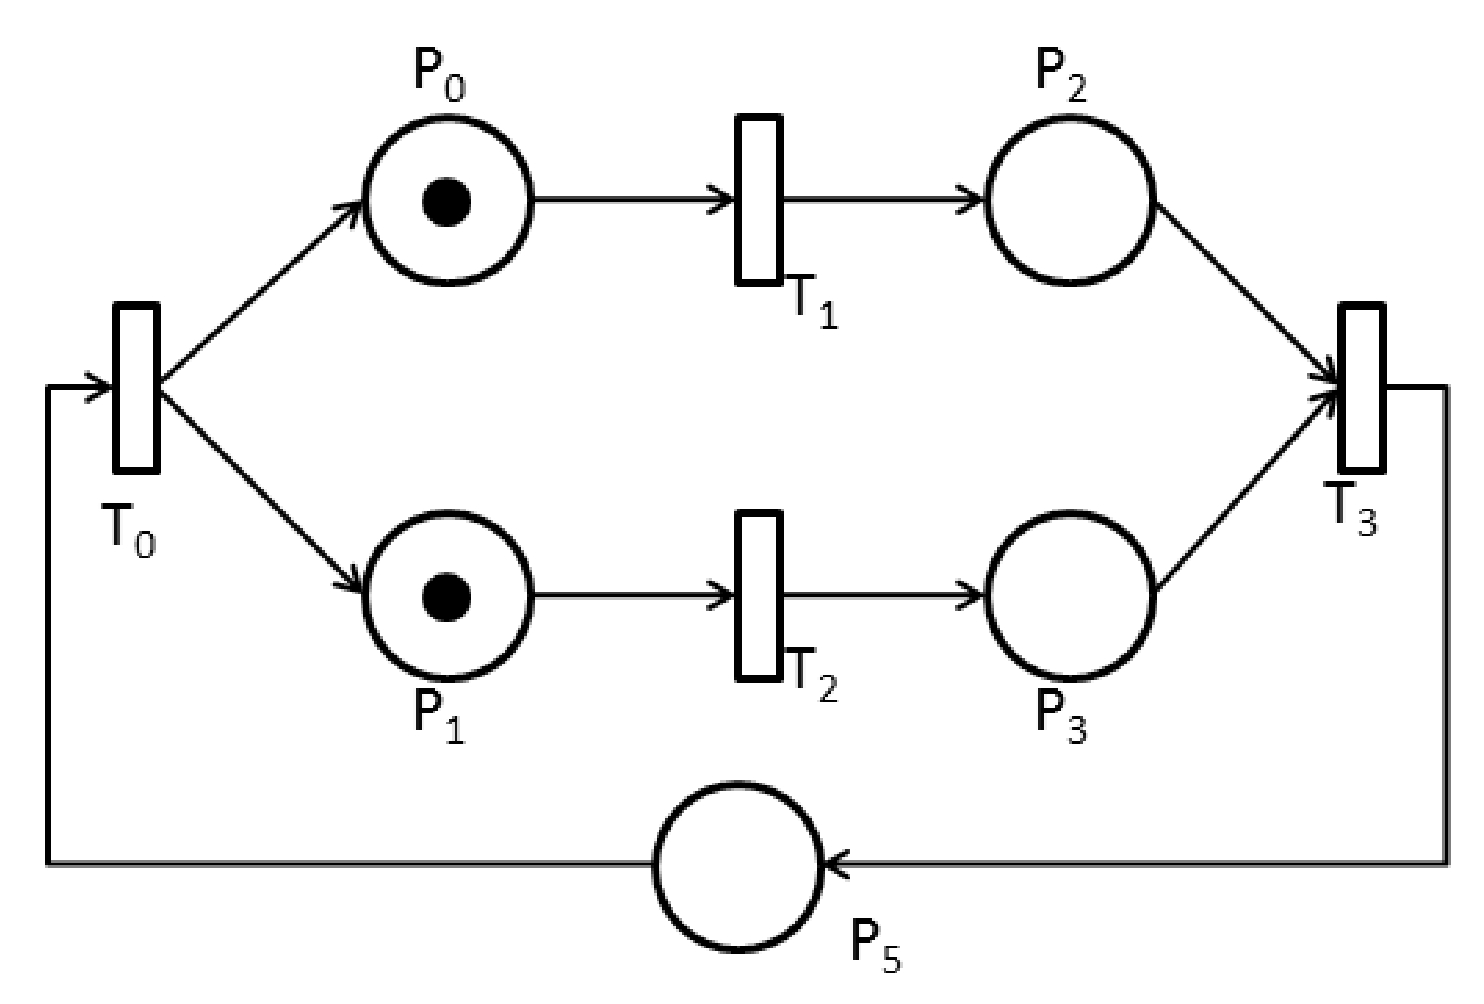
\includegraphics[width=4cm]{petri}};
		
		 % Labels:
		\fill[black]
			(-1,4) node[above=-3pt, scale=0.9] {\textsf{\bfseries Spécification du système}};	
	\end{scope}
	
	% vertical lines for linking agents on the 2 levels

	\draw[thick](-1.70,1.02) to[out=90,in=-90] (-1.70,-1);
	
	% User level
	\begin{scope}[
		yshift=0,
		every node/.append style={yslant=\yslant,xslant=\xslant},
		yslant=\yslant,xslant=\xslant
	]
		% The upper frame:
		\fill[white,fill opacity=.70] (-3.1,0) rectangle (3,6); % Opacity
		\draw[black, dashed, thick] (-3.1,0) rectangle (3,6); 
		 % Agents:
		\draw [fill=red]
			(-0.5,2) circle (.1); % .tex file

		% the icons
		\node[anchor=south,inner sep=0,xshift=-20pt,yshift=10pt,fill=white] at (1,2)
			{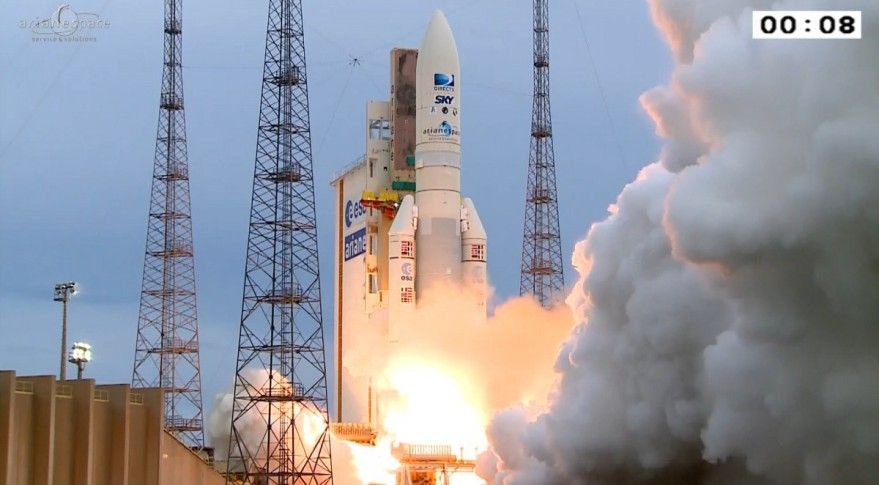
\includegraphics[width=4cm]{Ariane_5}};

		\fill[black]
			(-2,6) node[below right,,xshift=-20pt,yshift=-5pt,scale=.9,text width=2.5cm,align=left,fill=white]
				{\textsf{\bfseries \mbox{Système réel}}}		
		;
	\end{scope} 
	
		% vertical lines for linking agents on the 2 levels
	
	 \draw[thick](-1.70,-3	) -> (-1.70,-5);
	
	
		% system level
	\begin{scope}[
	yshift=-220,
	every node/.append style={yslant=\yslant,xslant=\xslant},
	yslant=\yslant,xslant=\xslant
	] 
	% The lower frame:
	\draw[dashed, thick,red] (-3,0) rectangle (3,4.8); 
	% Agents:
	\draw[fill=red]  
	(1.7,5.6) circle (.1); % .tex file
	% Flows:
	\node[anchor=south,inner sep=0,xshift=2pt,yshift=-5pt,fill=white] at (0,1)
	{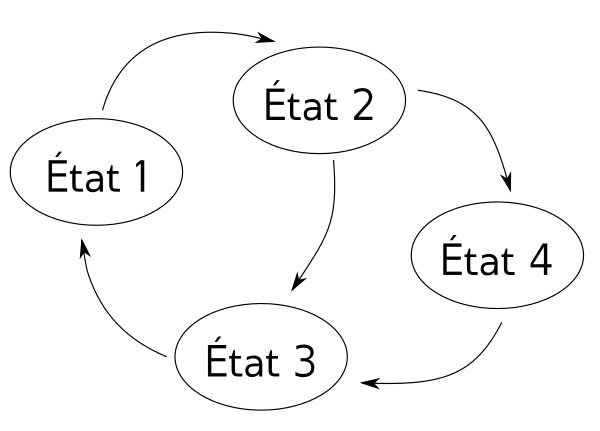
\includegraphics[width=4cm]{etats}};
	
	% Labels:
	\fill[black]
	(-1,4) node[above=-3pt, scale=0.9] {\textsf{\bfseries Espaces d'états}};	
	\end{scope}

	\begin{scope}[
	yshift=-20,
	xshift=200,
	every node/.append style={yslant=\yslant,xslant=\xslant},
	yslant=\yslant,xslant=\xslant
	] 
	% The lower frame:
	\draw[dashed, thick,green] (-3,0) rectangle (3,4.8); 
	% Agents:
	\draw[fill=green]  
	(-2,2) circle (.1); % .tex file
	\draw[thick](-2,2	) -> (-7,-2);
	% Flows:
	\node[anchor=south,inner sep=0,xshift=1pt,yshift=-10pt,fill=white] at (0,1)
	{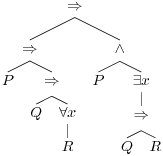
\includegraphics[width=4cm]{proposition}};
	
	% Labels:
	\fill[black]
	(-1,4) node[above=-3pt, scale=0.9] {\textsf{\bfseries Model checking}};	
	\end{scope}


	\begin{scope}[
		yshift=-100,
		xshift=250,
		every node/.append style={yslant=\yslant,xslant=\xslant},
		yslant=\yslant,xslant=\xslant
		] 
		% The lower frame:
		\draw[dashed, thick,fill=red,red] (-1,0) rectangle (1,1); 
		% Agents:
		\draw[black,fill=black]  
		(0,4) circle (.1); % .tex file
		\draw[thick,red](0,4) -> (0,0);
	
		
		% Labels:
		\fill[black]
		(0,0) node[above=-3pt, scale=0.9] {\textsf{\bfseries NON}};	
	\end{scope}

	\begin{scope}[
yshift=-150,
xshift=150,
every node/.append style={yslant=\yslant,xslant=\xslant},
yslant=\yslant,xslant=\xslant
] 
% The lower frame:
\draw[dashed, thick,fill=green,green] (-1,0) rectangle (1,1); 
% Agents:
  
\draw[thick,green](3.5,4) -> (0,0);


% Labels:
\fill[black]
(0,0) node[above=-3pt, scale=0.9] {\textsf{\bfseries OUI}};	
\end{scope}

\end{tikzpicture}
\end{document}